\chapter{Résultats et discussions}

Les expérimentations présentés précédemment nous ont permis de réunir, tester et sélectionner un ensemble d'outils et de méthodes déjà existants parmi ceux disponibles. Ces diverses tentatives ont notamment montrés les limites de chacune des approches, dégageant ainsi le champ pour la création d'un outil approprié à l'observation de la diffusion des mèmes sur les réseaux sociaux. 

Dans ce chapitre, nous décrirons tout d'abord dans le détail le fonctionnement de l'outil que nous avons choisi de développer : utilisation, choix technologiques, algorithmes et processus de validation. Ensuite, nous présenterons un ensemble de résultats obtenus grâce à cet outil par l'étude de figures réalisées autour d'une dizaine de mèmes sélectionnés. Au regard de ces résultats, nous discuterons des limites de ce type d'approche et plus largement des contraintes et écueils possibles de la méthodologique d'analyse de données.

\subsubsection{A propos des choix technologiques}

La conception et l'usage de technologies numériques se trouvant au cœur de cette recherche, nous avons été amené à effectuer de nombreux choix quant aux outils utilisés. Chacun des logiciels, programmes ou outils mobilisés sera présentés plus en détail dans les sections ci-dessous. Néanmoins, afin d'éclaircir le lecteur sur la nature et les raisons plus générales de ces choix, nous précisons ici les différents aspects qui sont entrés systématiquement en compte lors de chacun de  nos décisions :


\begin{description}
    \item[Licence : gratuité, open-source et disponibilité]
        La possibilité de lire, modifier et utiliser les outils et librairies dans le cadre de cette recherche est un des éléments primordiaux. Non seulement, les coûts de développement sont très largement diminuer par l'usage de solutions gratuites mais également la disponibilité des outils permet à ceux qui souhaiteraient se réapproprier les outils ou le code de le faire librement. De plus, le caractère \textit{open source} permet de consulter librement les rouages du code et s'assurer de sa validité et sa qualité avant de l'invoquer.

    \item[Documentation : communauté et support]
        Les outils parfois compliqués du développement informatique ne peuvent souvent être utilisés sans un minimum d'explication et de documentation. Si la documentation laisse à désirer, que le code est mal rédigé ou que la communauté des créateurs ou utilisateurs n'est pas présente procurer des explications, l'usage de technologies même très intéressante devient très difficile, voire impossible.

    \item[Interopérabilité : déploiement et compatibilité]
        Le degré de complexité des procédures d'installation et de mise en place de certaines technologies est également un facteur décisif dans la sélection d'un outil. En effet, la reproductibilité et la possibilité de réutilisation du code se voit très largement diminuée par un déploiement complexe et laborieux, multipliant souvent les erreurs. Les outils choisis pour ce travail ont été développé pour être compatibles uniquement avec le système d'exploitation Linux Debian, très largement répandu.

    \item[Validation : usage commercial et scientifique]
        Notre recherche ne se situe pas dans le domaine de la science informatique et à ce titre fait usage d'outils utilisés tant dans la communauté scientifique que dans l'industrie du Web. Le développement de nombreux  outils commerciaux s'originent dans la recherche scientifique. L'optimisation et la validation du code par les processus de contrôle de qualité de l'industrie sont également un facteur important dans la décision d'utiliser telle ou telle technologie.

\end{description}


\section{Un outil de traitement et de visualisation des mèmes}

Dans cette section, nous présenterons la structure et les développements spécifiques que nous avons mené pour construire cet outil. Les comment et pourquoi de nos différents choix technologiques seront explicités dans une présentation pas à pas du fonctionnement et de l'utilisation du système d'analyse que nous avons créé.

\subsection[Constitution de corpus par mots-clés pour chaque mème]{Constitution de corpus par mots-clés pour chaque mème}
\label{sec:keywords}

Comme nous l'avons vu précédemment,  ni les méthodes de détection algorithmiques (section \ref{sec:protomemes}) ni l'usage de l'objet hashtag (section \ref{sec:hashtags}) n'ont permis de saisir de manière satisfaisante l'objet mème dans le vaste jeu de données que nous avons choisi d'approcher (section \ref{sec:weiboscope}). 

Ainsi, nous avons choisi de considérer l'approche lexicale qui consiste à décrire le mème sous la forme de mots-clés. Pour chaque mème, nous procédons à l{\textquoteright}extraction d{\textquoteright}un jeu de données contenant l{\textquoteright}ensemble des messages correspondant à une requête définie composée de différents mots. 

La faiblesse intrinsèque de cette approche est néanmoins qu'elle nécessite de savoir ce qu'on veut chercher, à l'inverse d'une détection des mèmes qui permettrait de les identifier sans connaître leur existence a priori. Cette méthode prend peu en compte les éléments audio et visuels (images, vidéos) qui constituent pourtant une partie importante des mèmes constitués en ligne. 

Néanmoins, elle permet une approche intuitive par l'usage de mots-clés et une vérification itérative de la qualité des résultats obtenus, à l'inverse de la détection algorithmique notamment. Également, les faiblesses de la recherche plein-texte peuvent être contournées relativement facilement (effacement des éléments exogènes, complétion des corpus). 


\subsubsection[Indexation pour la recherche plein-texte]{Indexation du corpus Weiboscope pour la recherche plein-texte}

La fonction de recherche plein-texte est un des secteurs des technologies numériques qui a connu la plus forte expansion depuis les 10 dernières années de l'Internet, comme en témoigne l'histoire de \textit{Google}. L'accroissement des données et la nécessité de naviguer en leur sein ont fait des moteurs de recherche un élément incontournable du paysage de nos navigateurs. Chaque site web possède un champ "search" ou presque. Suivant cet important développement, des solutions de plus en plus fiables et performantes ont été mis à disposition sous des licences ouvertes, permettant facilement une appropriation.

Dans cette étude, nous avons choisi d'utiliser le moteur de recherche \textit{ElasticSearch}\footnote{Voir le site \url{http://www.elasticsearch.org}, consulté le 22 Avril 2014 à 12:23} pour accéder au contenu du corpus. Utilisant la très solide technologie du  moteur d'indexation \textit{Apache Lucene}  \footnote{ \url{http://lucene.apache.org/} consulté le 20 Juin 2014 à 11:22}, il permet d'indexer de larges corpus dans une base de données non-relationnelles, mettant à disposition une API efficace et structurée suivant la norme \textit{REST}. Largement utilisé et documenté, \textit{ElasticSearch} permet l'indexation des caractères chinois grâce au plugin Lucene \textit{SmartChinese Analyzer}. Ce plugin utilise un algorithme basé sur le modèle statistique dit de \textit{Modèle de Markov caché} appliqué à un vaste \textit{training corpus} de texte Chinois et de dictionnaires\footnote{Voir \url{http://www.ictclas.org/} consulté le 7 Juillet 2014 à 11:32} pour segmenter le texte chinois en mots. Les mots sont ensuite indexés dans la base de données de \textit{Lucene}. Chaque requête dans \textit{ElasticSearch} permet de comparer les instructions (mots-clés) aux documents textuels contenu dans la base de données, attribuant un poids spécifique à chaque document en fonction de la corrélation entre ses mots et ceux de la requête. Enfin, le moteur de recherche renvoie les résultats sous la forme d'un objet au format standard JSON qui permet sa réutilisation dans une interface pour l'interprétation des résultats obtenus.

Afin de procéder à la recherche de mème dans le texte, nous avons donc indexé dans \textit{ElasticSearch}les parties du corpus \textit{Weiboscope} à l'aide d'un script\footnote{consultable ici \url{https://github.com/clemsos/mitras/blob/master/es_build_index.py} consulté le 7 Juillet 2014 à 11:27}. Chacun des 52 fichiers au format \textit{zip} contenant des données au format \textit{csv} (texte des microblog en chinois et méta-données)  peut donc être déposé dans un dossier sélectionné pour être ensuite indexé. Cette manipulation est également reproductible pour tout type de fichiers en langue chinoise ou anglaise (d'autres langues nécessite l'ajout d'un simple analyseur de texte \textit{Apache Lucene}).

\subsubsection[Sélection qualitative de mots-clés]{Sélection qualitative de mots-clés}

Une fois le texte indexé, il nous faut maintenant définir les requêtes appropriés qui nous permettront d'extraire un corpus intéressant pour l'étude d'un ou plusieurs mèmes. La définition des mots-clés est un exercice compliqué dans de nombreux cas car il suppose que les mèmes ne recoupent pas ou peu des mots utilisés dans des sens multiples. Or, nous avons vu que le propre du mème est justement l'intertextualité et à ce titre joue littéralement sur les mots. Dans le contexte chinois, nous avons notamment vu l'exemple d'un mème construit autour des mots \textit{crabe de rivière} (voir figure \ref{fig:hexie}). Il y a de très fortes chances que les résultats d'un recherche pour les mots \textit{crabe} et \textit{rivière} dans le moteur de recherche et peu de lien avec ce mème somme toute très marginal dans la masse des contenus. Ici, la syntaxe propre du moteur de recherche peut nous venir en aide, permettant d'inclure (\textit{AND}) ou d'exclure (\textit{NO}) certains mots précis ou d'exiger du moteur de considérer des groupes de mots entier \textit{""}. Une autre possibilité est de limiter la recherche dans le temps en se concentrant sur une période donnée où le  mème connaît sa période de plus fort intérêt.

La qualité de la requête et des résultats renvoyés par le moteur de recherche pour chaque mème peut se définir  selon trois aspects importants :

\begin{description}
    \item[volume]
        Taille significative et volume suffisant de données pour constituer un corpus représentatif du mème.
    \item[qualité]
        Possibilité de vérifier manuellement la qualité du contenu par la lecture d{\textquoteright}un échantillon de  messages obtenus.
    \item[dimensions]
        Les différents paramètres retournés (dates, lieu, utilisateur précis, contenu censuré...) correspondent à ceux choisis dans la requête
\end{description}

La définition de la requête répondant au mieux aux besoins du chercheur  ne peut donc se faire a priori sans un certain nombre d'essais et tentatives. L'obtention de résultats satisfaisants passe par une phase itérative qui permet de définir et cerner une définition du mème sous forme d'une requête dans le moteur de recherche. Cette démarche implique non seulement la possibilité de pouvoir s'adonner à de multiples essais de formulations de la requête mais également la nécessité de lire les résultats sous une forme compréhensible. Si le format JSON reçu ou renvoyé par le moteur de recherche est un standard de l'échange de données, il n'est néanmoins pas adapté à la lecture et l'écriture par des humains. Ainsi, afin de pouvoir mener ce travail de façon intuitive et pratique, nous avons mis en place un tableau de bord à l'aide du logiciel \textit{Kibana} qui nous permet de contr\^oler la pertinence des résultats en comparant plusieurs requêtes différentes.

\begin{figure}[h!]
    \centering
    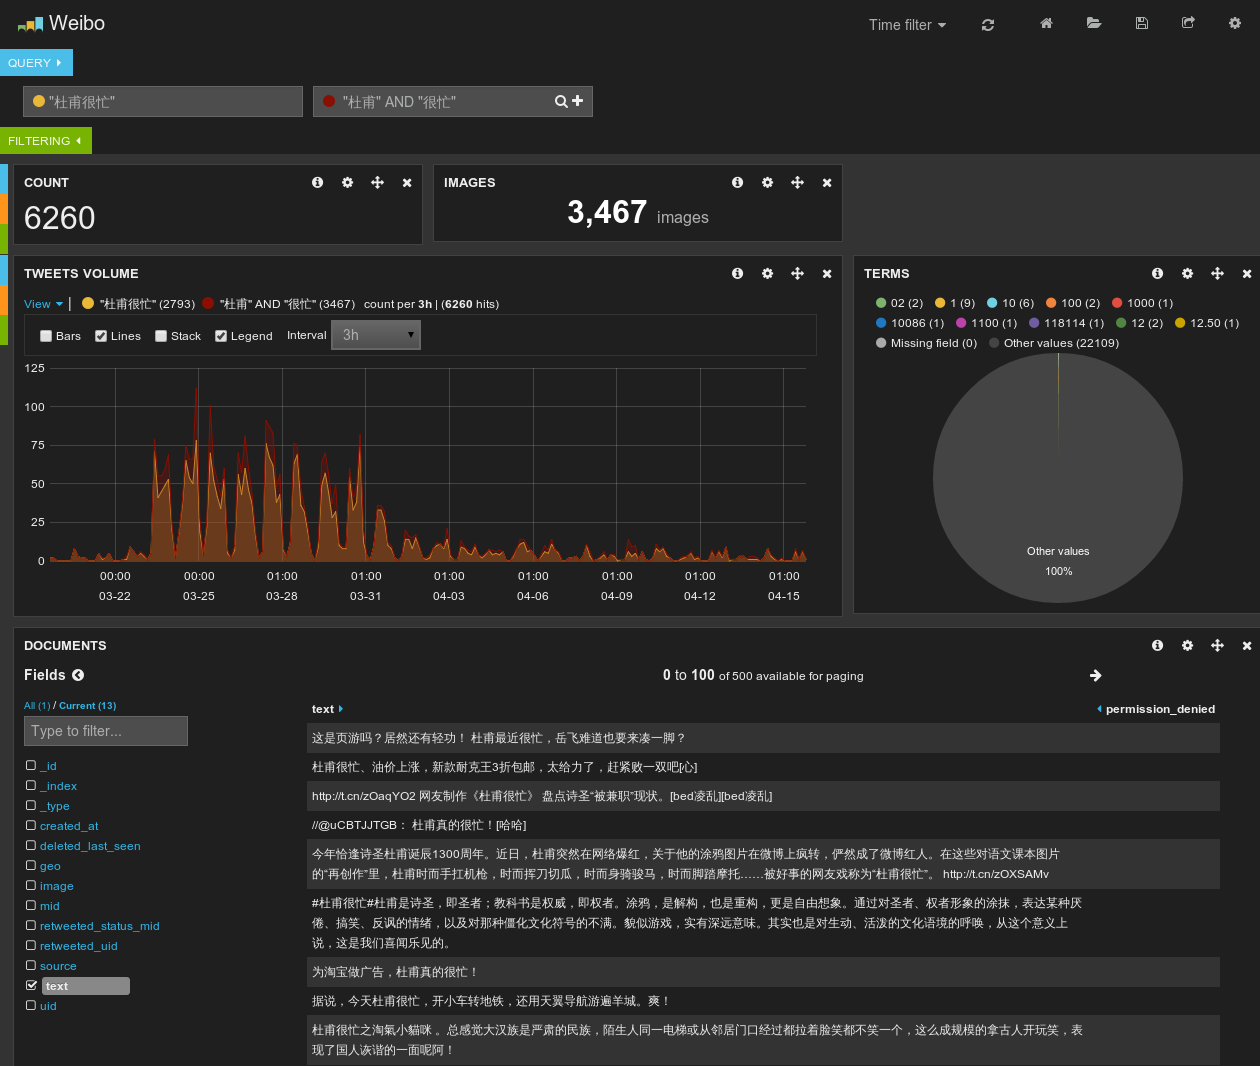
\includegraphics[width=6.0004in,height=5.078in]{figures/chap3/chapitre3-img20.png}
    \caption[Tableau de bords requêtes par mots-clés] { Ce tableau de bord permet de comparer la qualité de différentes requ\^etes dans le corpus. Capture d'écran réalisée le 23 Mars 2014 à 16h18}
\end{figure}

\subsubsection[Constitution d'un corpus pour chaque mème]{Constitution d'un corpus pour chaque mème}


En contrôlant la qualité de ses différents critères nous pouvons donc identifier une requête adéquate pour décrire le mème. Une fois cette étape effectuée, nous procédons à l'extraction des messages qui vont venir constituer le corpus d'études de notre mème. Pour s'assurer de la fiabilité des résultats, nous disposons de l'index de poids du moteur de recherche qui représente la similarité entre notre requête et les messages obtenus. Pour limiter le nombre de résultats, nous pouvons fixer un poids minimum (par exemple 0,5) et ainsi limiter le bruit en ignorant les messages sans lien avec notre requête.

Une fois extrait, ce jeu de données est stocké dans un fichier de type  \textit{csv} respectant le format initial et l'encodage des données de Weiboscope. Afin de parfaire la complétude de ce jeu de données, les messages mentionnés et les retweets ne contenant pas le mot clé (commentaires, réponses, etc.) sont rassemblés pour donner finalement un ensemble de messages représentatifs du mème qui va pouvoir être analysé.

\subsection[Extraction des graphes et traitement des données]{Extraction des graphes et traitement des données}

L{\textquoteright}étude des relations entre ces différents types d{\textquoteright}espaces implique donc une méthodologie renouvelée et le développement d{\textquoteright}outils adaptés. Il ne s{\textquoteright}agit plus simplement d{\textquoteright}étudier un réseau, mais plus précisément de s{\textquoteright}interroger sur les relations entre différents réseaux, de nature souvent différentes. Au-delà du réseau multi-calques, nous sommes en présence de multiples réseaux possédant des relations communes. 

Nous avons donc sélectionné trois aspects importants des mèmes que nous allons tenter de représenter au mieux afin d{\textquoteright}en comprendre l{\textquoteright}existence :

\begin{description}
\item[Langagier] Le champ sémantique d{\textquoteright}un mème est constitué des mots qui sont prononcés lors de sa diffusion. L{\textquoteright}association de mots -souvent sous la forme du jeu de mots - est un des propres du mème et constitue ainsi une part importante de son existence. Ainsi, le mème produit à proprement parler des réseaux de mots en dessinant des liens entre des signifiants souvent improbables qui en font souvent le succès \citep{Bauckhage2011}. 

\item[Conversationnel] Plus que les mots, un mème se constitue sous la forme d{\textquoteright}un échange, une conversation o\`u les différents acteurs discutent, commentent et se saisissent des actions disponibles sur la pateforme web (like, retweets, etc.) pour converser. Comme nous l{\textquoteright}avons vu précédemment, nous pouvons identifier et considérer un graphe conversationnel créé par le mème en se diffusant. 

\item[Réel] Au-delà des échanges en ligne, ces discussions possèdent une existence physique, premièrement sous la forme de l{\textquoteright}activité électrique des machines qui sont utilisées lors de ce processus. Néanmoins, dans l{\textquoteright}approche d{\textquoteright}une géographie humaine des échanges numériques, nous considérerons ici l{\textquoteright}existence physique des mèmes par celle des utilisateurs - de leurs corps - et non pas des machines. 
\end{description}


Afin d{\textquoteright}étudier chacun de ces aspects du mème, nous allons donc procéder à la collection et la visualisation de données sur chacun de ces niveaux d{\textquoteright}après un corpus de mèmes sélectionnés. 


Nous procédons ensuite au traitement de chaque corpus selon une
série de procédures définies comme suit :

\subsubsection{Graphe lexical}

Le texte de chaque message est analysé de fa\c{c}on à ne conserver
que les mots les plus importants. Cela s{\textquoteright}effectue en
cinq étapes successives : 

\begin{enumerate}
\item La phrase est segmentée (analyse de la langue chinoise) pour
obtenir un ensemble de mots du mème.
\item A chacun des mots est associé l{\textquoteright}ensemble des
utilisateurs l{\textquoteright}ayant mentionné.
\item Les mots les plus courants sont enlevés afin de réduire le
bruit. La constitution de la liste des mots courants
\textit{(stopwords) }est une étape très importante. La liste que
nous utilisons a été créée à partir de différents corpus
lors d{\textquoteright}expérimentations précédentes et
augmentée de nouveaux mots au fur et à mesure.
\item La co-occurence d{\textquoteright}un mot dans une même phrase
définit une relation entre ces deux mots.
\item Parmi l{\textquoteright}ensemble de mots-clés ainsi obtenu, nous
conservons les 500 mots les plus utilisés (dont les occurences sont
les plus nombreuses) 
\item Nous reconstituons le graphe des relations entre ces 500
mots-clés d{\textquoteright}après la série de leur co-occurence :
chaque mot est un node, chaque co-occurence est un edge.
\item L{\textquoteright}ensemble constitue le graphe sémantique du
mème, pondéré mais non dirigé.
\end{enumerate}

\subsubsection{Graphe conversationnel}

Pour chaque mème, l{\textquoteright}ensemble des interactions
(mentions, citations et retweets) consituent le graphe conversationnel
o\`u un utilisateur est un node et une interaction est un edge. Le
graphe est dirigé car les interactions vont depuis un utilisateur à
un autre. 

Une fois l{\textquoteright}ensemble du graphe constitué, nous
déterminons sa modularité et son coefficient moyen de clustering
afin de posséder des informations sur sa structure. Nous calculons
également la centralité intermédiaire (\textit{betweenness
centrality}) pour chaque utilisateur dans l{\textquoteright}ensemble du
graphe. Ensuite, nous identifions les différentes communautés en
utilisant l{\textquoteright}algorithme dit de Louvain et son
implémentation par Blondel \& al. \citep{Blondel2008}\footnote{
\url{http://perso.crans.org/aynaud/communities/index.html} consulté
le 22 Avril 2014 à 14:24} qui nous permet d{\textquoteright}attribuer
à chaque utilisateur un groupe unique. Enfin, nous réduisons la
taille du graphe final en ne conservant que les utilisateurs ayant
effectué au moins 2 échanges - en supprimant les \textit{edges} du
graphe ayant un poids inférieur à 2.

Le graphe ainsi constitué correspond aux données conversationnelles
du mème.

Le détail de l'algorithme utilisé pour produire les graphes conversationnels et lexicaux est disponible dans les annexes de ce document à la référence \ref{algo:meme-graph}

\subsubsection{Localisation des utilisateurs}

Pour chaque mème, nous souhaitons également regrouper les
informations de localisation des utilisateurs mentionnés ou actifs
dans le mème. Le jeu de données \textit{Weiboscope }comprend les
localités mentionnées par les utilisateurs dans leurs profils. Le
nombre de ces localités est restreinte par
l{\textquoteright}interface de Sina Weibo elle-même à :
l{\textquoteright}ensemble des provinces de Chine continentale, Hong
Kong, Macau, Taiwan, {\textquotedblleft}à
l{\textquoteright}étranger{\textquotedblright} et
{\textquotedblleft}autres{\textquotedblright}. Ainsi, pour chaque
utilisateur nous assignons l{\textquoteright}information géographique
mentionnée par l{\textquoteright}utilisateur dans son profil.

\subsection{Serveur et moteur de visualisation interactive}

Une fois que l{\textquoteright}ensemble de ces données a été extrait et traité, nous pouvons considérer différents aspects au sein du mème :

\begin{description}
\item[Graphe sémantique] mots-clés et relations entre les mots
\item[Graphe socio-sémantique] relations entre les mots et les
utilisateurs
\item[Graphe conversationnel] relations et communautés
d{\textquoteright}utilisateurs 
\item[Graphe socio-géographique] relations entre les utilisateurs et
les provinces / villes chinoises
\end{description}

Nous avons donc plusieurs niveaux de lecture interdépendants qui nous permettent de considérer différents aspects de chaque mème. Néanmoins, les informations de graphe sont peu claires et difficilement exploitables sous forme de données, à l{\textquoteright}exception d{\textquoteright}une série de mesures indicatives sur leurs structures. Afin d{\textquoteright}explorer ces différentes relations, il nous faut pouvoir visualiser différentes dimensions du mème afin d{\textquoteright}observer les articulations et phénomènes possibles émergents de cette lecture. 

Pour réaliser cette cartographie particulière, il n{\textquoteright}existe pas d{\textquoteright}outils disponibles permettant de mettre en relation différents types de réseaux. Nous avons donc choisi de développer une solution technologique adaptée à nos besoins permettant de considérer sous différents angles l{\textquoteright}ensemble de ces graphes et de leurs relations. Les différents choix conceptuels et technologiques présidant au design de cet outil de visualisation sont détaillés ci-après. 


Egalement,
l{\textquoteright}ensemble de l{\textquoteright}outil de visualisation
se fonde sur HTML5, CSS3 et Javascript qui sont des langages ouverts
issues d{\textquoteright}un travail collectif de
l{\textquoteright}ingénierie du Web permettant la réutilisation
partielle ou totale des travaux produits par d{\textquoteright}autres
et contribuant ainsi à davantage
d{\textquoteright}interopérabilité entre les différents design
scientifiques de recherche. La mise en forme des données utilise la
librairie {\textquotedblleft}Data-Driven Documents{\textquotedblright}
(d3.js)\footnote{ D3js at \url{http://d3js.org/,} consulté le 24
Avril 2014 à 14:58}, les données elles-mêmes sont stockées en
JSON pour les graphes et GeoJSON pour les données cartographiques.

\subsubsection{Espace perceptif, plan projectif et choix d{\textquoteright}un {\textquotedblleft}layout{\textquotedblright}}

Devant la disparité des données en présence, nous devons donc
construire un espace de représentation ou plut\^ot une interface de
représentation propice à l{\textquoteright}exploration et la
découverte des phénomènes dans les relations entre les
différents graphes. Dans la définition de cet espace perceptif se
joue la réconciliation d{\textquoteright}entités dissemblables (des
utilisateurs, des lieux, des mots, leurs relations mutuelles). La
t\^ache consisterait ainsi à réconcilier dans le plan de
l{\textquoteright}espace graphique de la visualisation (ici celui de
l{\textquoteright}écran) les différents espaces o\`u projeter ces
différents graphes. A l{\textquoteright}image du milieu numérique,
l{\textquoteright}existence même de ce plan réconciliant global,
local, réel, symbolique et imaginaire pose question. A la simple
question : {\textquotedblleft}quelle doit être sa
couleur?{\textquotedblright}, une logique commune de lisibilité
répondrait : {\textquotedblleft}blanc ou noir{\textquotedblright},
mais quelle peut en être la justification logique dans
l{\textquoteright}espace de la visualisation? Et que penser du coté
de l{\textquoteright}écran? De quoi est-t-il le bord? Dès lors que
se pose la question de structurer un espace de perception, nous voilà
devant plusieurs difficultés formelles majeures.
L{\textquoteright}exigence de rigueur scientifique et surtout
l{\textquoteright}imperméabilité des formats de publications
scientifiques actuelles rajoutent à la compexité de cette
entreprise.

Afin de pouvoir considérer les relations entres mots, communautés et
territoires, nous devons dans l{\textquoteright}espace graphique
disponible, il est nécessaire de résoudre plusieurs problèmes :

\begin{itemize}
\item Donner à voir chaque type d{\textquoteright}entités de
fa\c{c}on reconnaissable (provinces chinoises, communautés, mots)
\item Donner à voir les relations entre les différentes entités
(graphe multiples)
\item Pallier l{\textquoteright}augmentation de la complexité visuelle
et préserver une lisibilité
\end{itemize}
Nous avons donc choisi de construire un espace sur plusieurs niveaux
hiérachisés.

\subsubsection{Graphes et interactions}

Le centre de la visualisation est occupé par les utilisateurs,
reflétant à la fois l{\textquoteright}intérêt central de cette
étude pour l{\textquoteright}étude des processus
d{\textquoteright}individuation et le r\^ole charnière des
utilisateurs dans la structuration des données. Plus exactement, nous
avons choisi de regrouper les utilisateurs par communautés afin de
considérer les liens qui les unissaient entre elles et la structure
générale de la discussion plut\^ot que de
s{\textquoteright}intéresser aux individus. Les individus sont
symbolisés par des points au sein des communautés dont la couleur
indique leur centralité dans le réseau global. 

Notre première idée a été de représenter
l{\textquoteright}ensemble des utilisateurs sur une carte pour
comprendre comment s{\textquoteright}agencaient spatialement chacune
des discussions. La première étape a donc été de reconstituer
une carte de la Chine comprenant Taiwan, Hong Kong et Macau. Chacun de
ces territoires possèdent une influence médiatique certaine en
Chine et méritent à ce titre d{\textquoteright}être
représenté. Néanmoins, le statut politique particulier de chacun
de ces territoires nous a obligé à reconstituer une carte o\`u ils
figuraient tous. Nous avons choisi d{\textquoteright}aggrandir
l{\textquoteright}échelle de Hong Kong et Macau afin
qu{\textquoteright}il soit visible sur la carte. Egalement, nous avons
choisi de ne pas restituer les données concernant les utilisateurs
ayant choisi {\textquotedblleft}autres{\textquotedblright} ou
{\textquotedblleft}reste du monde{\textquotedblright} comme leurs lieux
de résidence.

Si la carte se prête assez bien à la visualisation de quantité,
les visualisations de graphe deviennent facilement confuses. Ainsi,
nous avons choisi d{\textquoteright}ajouter une option de visualisation
des provinces sous la forme d{\textquoteright}une liste, au moins toute
aussi parlante. Cela nous permet en plus d{\textquoteright}organiser
cette liste selon différents critères afin
d{\textquoteright}étudier plusieurs aspects qui peuvent être
intéressants.

Le graphe de mots revêt ici la forme la plus simple. Les relations
entre les mots sont matérialisées par un graphe utilisant un
algorihme force-based pour disposer les mots entre eux, recréant
ainsi des groupes de mots intéressants d{\textquoteright}après leur
proximité dans les phrases lors des discussions. Un positionnement
des mots selon leur importance (nombre de citations) est également
disponible à loisir.

Afin d{\textquoteright}explorer les différentes dimensions du graphes,
nous avons également ajouté des interactions qui permettent de
focaliser sur des zones ou des caractéristiques précises des
graphes. \citep{Bostock2011}

\begin{figure}
\centering
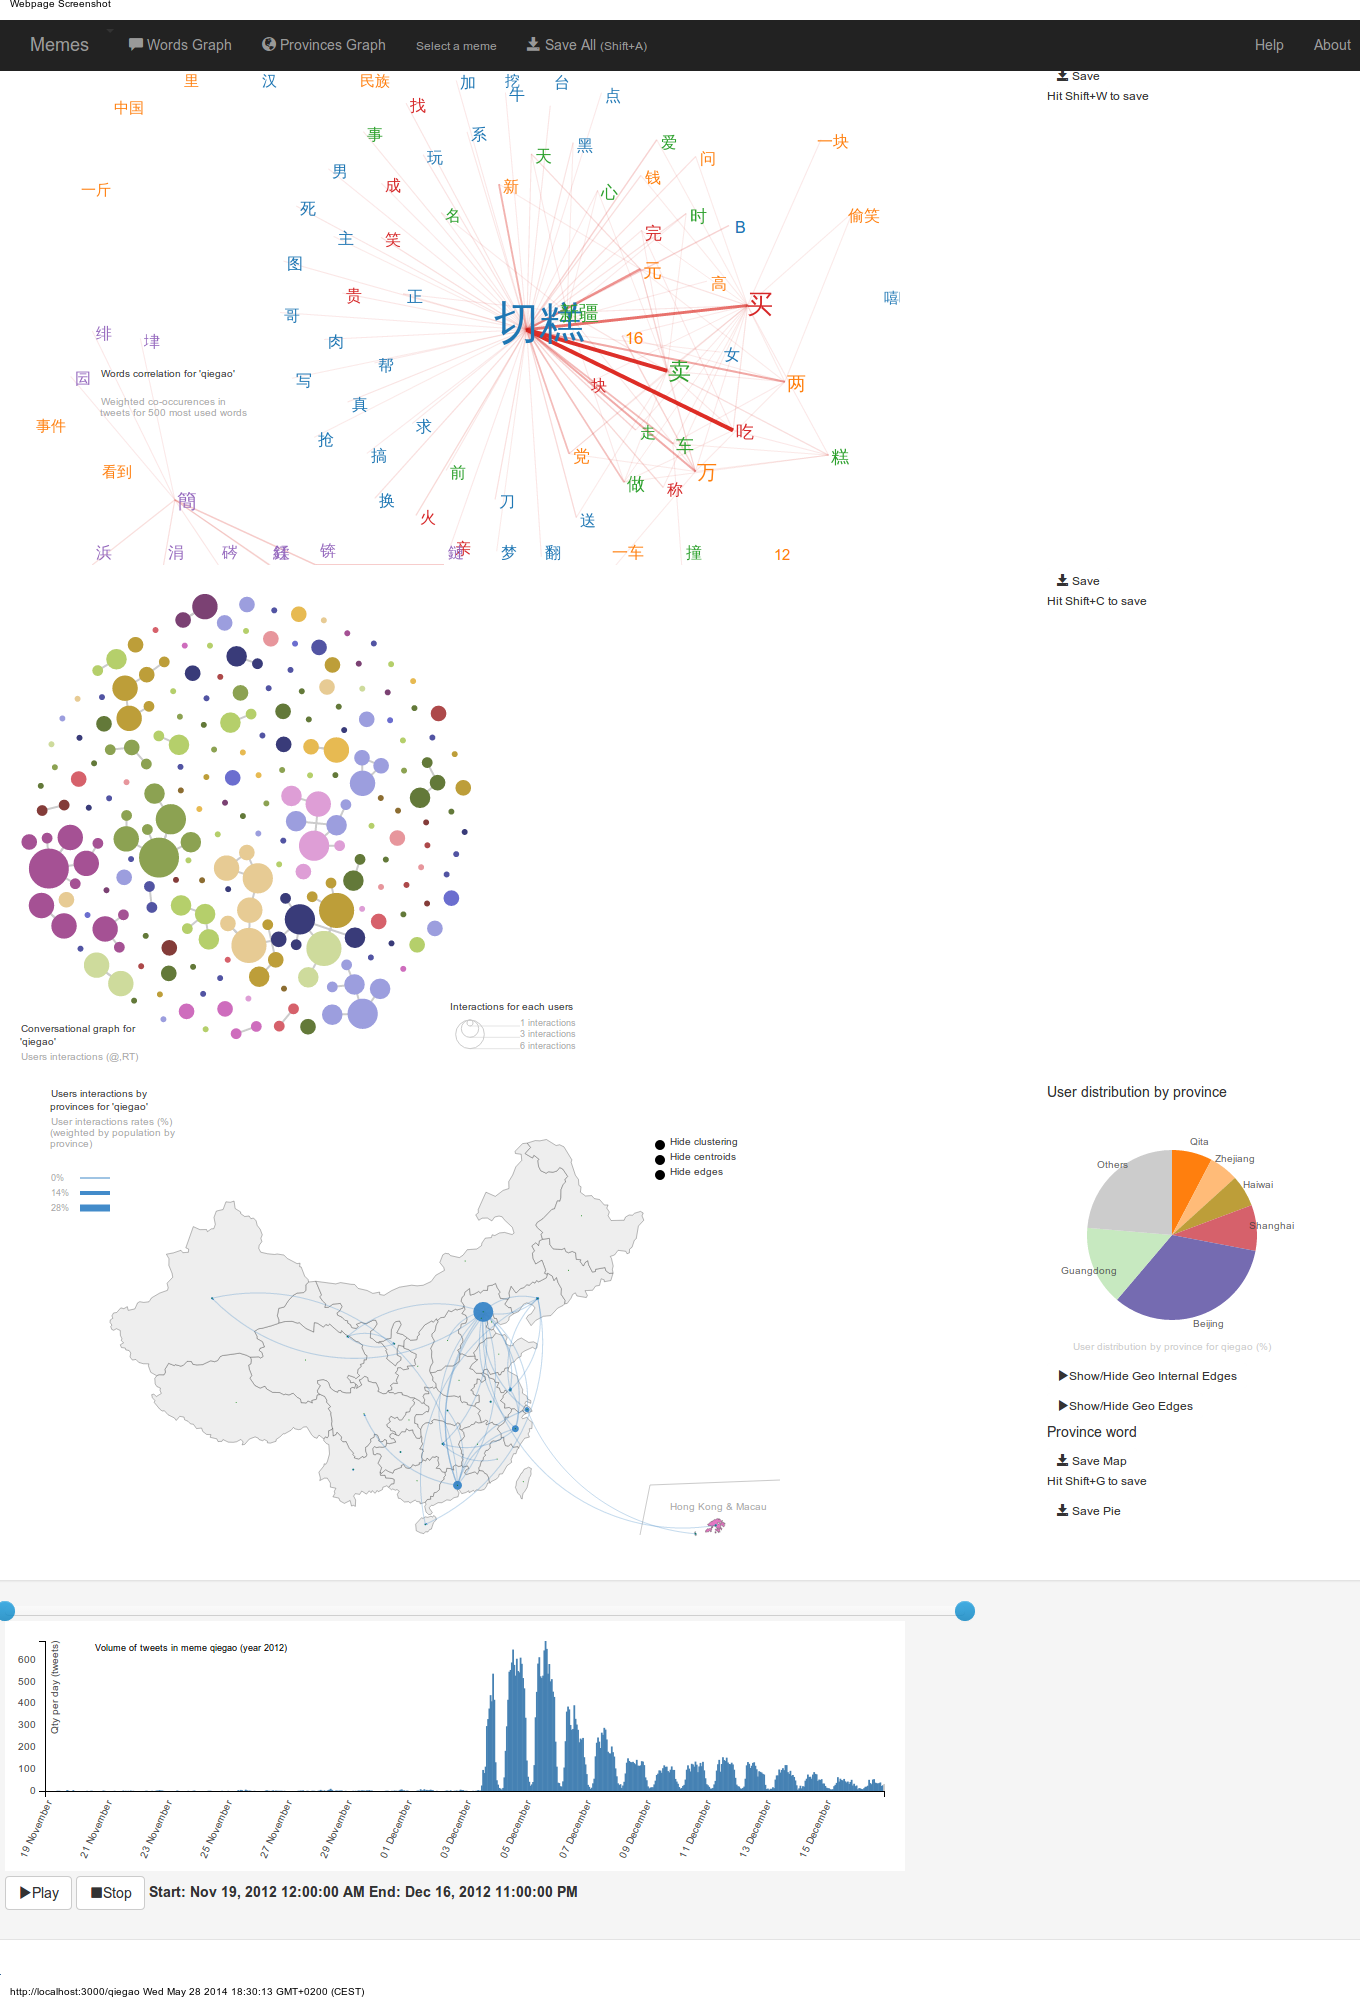
\includegraphics[width=6.7213in,height=8.3894in]{figures/chap3/chapitre3-img21.png}
\caption{Interface d'exploration et de visualisation des données}
\end{figure}


\subsection[Validité et validation de l outil]{Validité et validation de l outil}

validité interne/externe (Tannery)